% =====================================================================
%  EnergyMind Tunisia -- Goal 1, Phase 1 technical note:
%  Anomaly Detection for a Trustworthy Smart-Metered Grid.
%
%  All plots are drawn by PGFPlots from the data files in ./data.  gen.py
%  produces the illustrative figures (synthetic, fixed seeds); n1_experiment.py
%  produces the Section 5 results on node N1 of the EnergyMind dataset.
%  data/numbers.tex and data/n1_*.tex hold every number quoted in the text.
%  Build:  python gen.py && python n1_experiment.py && pdflatex main.tex (x2)
% =====================================================================
\documentclass[11pt,a4paper]{article}
\usepackage[utf8]{inputenc}
\usepackage[T1]{fontenc}
\usepackage{lmodern}
\usepackage[margin=2.5cm]{geometry}
\usepackage{amsmath,amssymb}
\usepackage{booktabs,tabularx,array}
\usepackage{listings}
\usepackage[table]{xcolor}
\usepackage{tikz}
\usetikzlibrary{arrows.meta,positioning}
\usepackage{pgfplots}
\pgfplotsset{compat=1.18}
\usepgfplotslibrary{groupplots}
\usepackage{enumitem}
\usepackage{needspace}
\usepackage{float}
\usepackage{subcaption}
\usepackage[hidelinks]{hyperref}
\newcolumntype{L}{>{\raggedright\arraybackslash}X}
\lstset{basicstyle=\ttfamily\footnotesize,breaklines=true,frame=single,
        columns=fullflexible,keepspaces=true,backgroundcolor=\color{black!3},
        xleftmargin=2pt,xrightmargin=2pt}

% generated by gen.py -- do not edit
\newcommand{\zOrd}{1.6, 3.1, 4.0, 4.9}
\newcommand{\zRob}{4.2, 7.7, 9.9, 12.0}
\newcommand{\zOrdHidden}{1}
\newcommand{\cusumAlarm}{84}
\newcommand{\cusumDelay}{4}
\newcommand{\ifOutMin}{0.63}
\newcommand{\ifOutMax}{0.77}
\newcommand{\ifNormMean}{0.46}
\newcommand{\ifSMin}{0.40}
\newcommand{\ifSMax}{0.80}
\newcommand{\pathNormal}{11.6}
\newcommand{\pathAnom}{5.2}

% generated by n1_experiment.py -- do not edit
\newcommand{\nOneDays}{10{,}715}
\newcommand{\nOneClean}{9{,}494}
\newcommand{\nOneEvents}{74}
\newcommand{\stackFPR}{2.3}
\newcommand{\gapSd}{0.6}
\newcommand{\balFPR}{5.2}
\newcommand{\nRare}{16}
\newcommand{\nRareHit}{9}


% colours of the figures
\definecolor{mzteal}{RGB}{15,118,110}
\definecolor{mzorange}{RGB}{230,135,30}
\definecolor{mzred}{RGB}{190,50,40}
\definecolor{mznavy}{RGB}{30,58,95}
\definecolor{good}{RGB}{170,215,208}
\definecolor{fair}{RGB}{248,218,180}
\definecolor{poor}{RGB}{240,205,205}

% heat cell for Table 3: shade proportional to recall, white text when dark
\newcommand{\hc}[1]{\expandafter\hcaux\expandafter{\the\numexpr #1*8/10\relax}{#1}}
\newcommand{\hcaux}[2]{\cellcolor{mzteal!#1}\ifnum #2>55 \textcolor{white}{#2}\else #2\fi}

\pgfplotsset{
  mz/.style={width=4.3cm,height=3.4cm,tick label style={font=\tiny},
    label style={font=\scriptsize},title style={font=\scriptsize\bfseries},
    grid=major,grid style={black!10},xmin=0,xmax=72,xtick={0,24,48,72}},
  colormap/ifmap/.style={colormap={ifmap}{rgb255=(255,248,238) rgb255=(245,190,120)
    rgb255=(230,135,30) rgb255=(200,80,30) rgb255=(150,40,30)}},
  colormap/svmmap/.style={colormap={svmmap}{rgb255=(150,40,30) rgb255=(200,80,70)
    rgb255=(255,255,255) rgb255=(120,200,185) rgb255=(15,118,110)}},
}


\title{EnergyMind Tunisia -- Goal 1\\[2pt]\large Anomaly and Bias Detection for a Trustworthy Smart-Metered Grid}
\author{}
\date{\small Phase 1 technical note: types of anomalies, families of detectors, what we use, and why.\\
All figures are generated from code (data files + TikZ/PGFPlots).}

\begin{document}
\maketitle

\paragraph{In one paragraph.} Our system must decide, for every suspicious reading, whether the \emph{grid}
did something unusual or the \emph{data} is wrong, because the two need opposite responses. No single
detector can do this. We therefore combine (i) physics and statistical rules, which are auditable,
(ii) three unsupervised machine-learning detectors trained only on clean data, which are sensitive to subtle
patterns, and (iii) a cross-sensor consistency reasoner that separates genuine events from data-quality
problems. Section~\ref{sec:stack} tests the detection layers on node N1 of the EnergyMind dataset and
reports, per fault type, what they catch and what they still miss.

% =====================================================================
\section{The Problem: a Suspicious Number Has Two Possible Meanings}
\label{sec:problem}
An anomaly is a pattern that deviates from expected behaviour~\cite{chandola}. In our prototype node (N1 of
the EnergyMind dataset: one transformer, 30 smart meters on 3 low-voltage feeders of 10, three homes with
rooftop PV, readings every 30~minutes, each feeder metered at its head) a surprising value can come from the
\textbf{grid} or from
the \textbf{data chain}, and the right response differs: a real event needs operational action, a faulty or
falsified sensor needs to be distrusted and repaired. A further difficulty is that an informed attacker can
craft false data that passes standard bad-data checks~\cite{fdi}, so one test is never enough.

\begin{figure}[H]
\centering
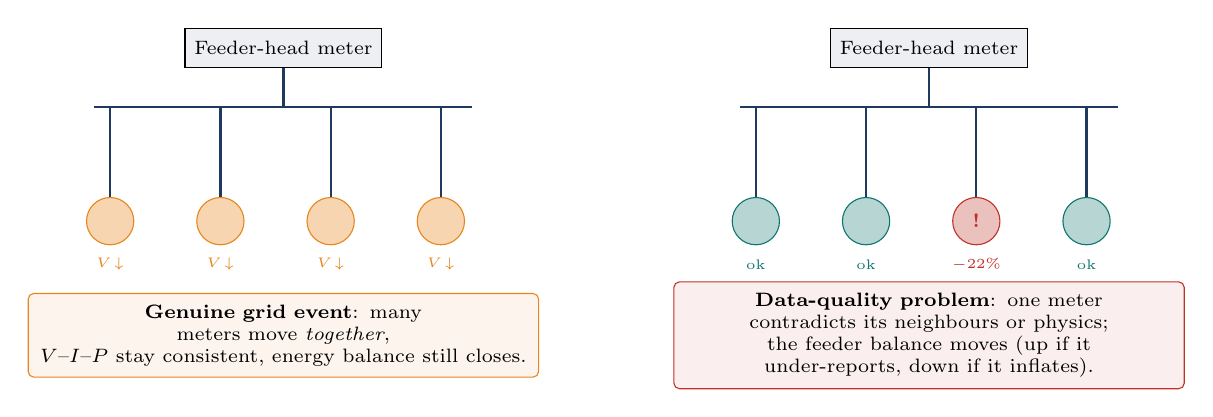
\begin{tikzpicture}[
  meter/.style={circle,draw,minimum size=6mm,inner sep=0pt,font=\scriptsize\bfseries},
  head/.style={draw,fill=mznavy!8,font=\scriptsize,minimum height=5mm},
  note/.style={draw,rounded corners=2pt,font=\scriptsize,align=center,text width=62mm,inner sep=4pt}]
\foreach \side/\x in {L/0,R/8.2}{
  \node[head] (h\side) at (\x+3,2.2) {Feeder-head meter};
  \draw[mznavy,thick] (h\side.south)--(\x+3,1.45);
  \draw[mznavy,thick] (\x+0.6,1.45)--(\x+5.4,1.45);
}
\foreach \x in {0.8,2.2,3.6,5.0}{\draw[mznavy,thick] (\x,1.45)--(\x,0.3);}
\foreach \x in {9.0,10.4,11.8,13.2}{\draw[mznavy,thick] (\x,1.45)--(\x,0.3);}
% left: genuine event, every meter sees the same voltage dip
\foreach \x in {0.8,2.2,3.6,5.0}{
  \node[meter,fill=mzorange!35,draw=mzorange] at (\x,0) {};
  \node[font=\tiny,text=mzorange] at (\x,-0.55) {$V\!\downarrow$};}
% right: data-quality problem on a single meter
\foreach \x in {9.0,10.4,13.2}{
  \node[meter,fill=mzteal!30,draw=mzteal] at (\x,0) {};
  \node[font=\tiny,text=mzteal] at (\x,-0.55) {ok};}
\node[meter,fill=mzred!30,draw=mzred,text=mzred] at (11.8,0) {!};
\node[font=\tiny,text=mzred] at (11.8,-0.55) {$-22\%$};
\node[note,fill=mzorange!8,draw=mzorange] at (3,-1.45)
  {\textbf{Genuine grid event}: many meters move \emph{together},\\ $V$--$I$--$P$ stay consistent, energy balance still closes.};
\node[note,fill=mzred!8,draw=mzred] at (11.2,-1.45)
  {\textbf{Data-quality problem}: one meter contradicts its neighbours or physics;\\ the feeder balance moves (up if it under-reports, down if it inflates).};
\end{tikzpicture}
\caption{The core question. Left: a real event is visible on many sensors and obeys physics. Right: a faulty
or falsified channel disagrees with redundant measurements. This cross-sensor logic is the backbone of our
design.}
\label{fig:core}
\end{figure}

% =====================================================================
\section{Types of Anomalies}
\label{sec:types}
The literature classifies anomalies by how they relate to context~\cite{chandola}. We use that
classification and map it onto grid failures (Figure~\ref{fig:types}, Table~\ref{tab:taxonomy}).

\begin{figure}[H]
\centering
\begin{tikzpicture}
\begin{groupplot}[group style={group size=4 by 1,horizontal sep=7mm},mz,xlabel={hours}]
\nextgroupplot[title={Point},ylabel={$V$},ymin=225,ymax=249]
  \addplot[black!35,thin] table[x=t,y=v]{data/types_point.dat};
  \addplot[mzred,only marks,mark=diamond*,mark size=2pt] table[x=t,y=anom]{data/types_point.dat};
  \addplot[mzred,only marks,mark=diamond*,mark size=2pt] table[x=t,y=ref]{data/types_point.dat};
\nextgroupplot[title={Contextual},ymin=225,ymax=249]
  \addplot[black!35,thin,unbounded coords=jump] table[x=t,y=v]{data/types_context.dat};
  \addplot[mzred,only marks,mark=*,mark size=1.6pt] table[x=t,y=anom]{data/types_context.dat};
  \draw[mzred,thick,-{Stealth[length=1.5mm]}] (axis cs:27,227.3)--(axis cs:27,231.6);
\nextgroupplot[title={Collective (stuck)},ymin=225,ymax=249]
  \addplot[black!35,thin,unbounded coords=jump] table[x=t,y=v]{data/types_stuck.dat};
  \addplot[mzred,thick,const plot,unbounded coords=jump] table[x=t,y=anom]{data/types_stuck.dat};
\nextgroupplot[title={Collective (drift)},ymin=225,ymax=244]
  \addplot[black!35,thin] table[x=t,y=v]{data/types_drift.dat};
  \addplot[mzorange,thick,unbounded coords=jump] table[x=t,y=anom]{data/types_drift.dat};
\end{groupplot}
\end{tikzpicture}
\caption{Illustrative voltage traces (synthetic, 30-min samples as in the dataset). Grey: normal behaviour. Red/amber: the
anomaly. A \emph{point} anomaly is one odd value; a \emph{contextual} anomaly is a value that is normal in
general but wrong for its time of day; \emph{collective} anomalies are odd only as a sequence (a frozen
sensor, a slow drift).}
\label{fig:types}
\end{figure}

\begin{table}[H]
\centering
\small
\begin{tabularx}{\textwidth}{@{}>{\raggedright\arraybackslash}p{3.1cm}>{\raggedright\arraybackslash}p{2.3cm}LL@{}}
\toprule
\textbf{Project anomaly} & \textbf{Type~\cite{chandola}} & \textbf{Signature in the data} & \textbf{First line of defence} \\
\midrule
Impossible value (spike, sign or unit error, saturation) & Point & $E<0$, $E=99.999$, $\times1000$, $\times8$--$40$ & Range rules \\
Stuck meter & Collective & Every channel frozen ($E$ \emph{and} $V$) & Flat-line rule \\
Data-only injection (scale, evasion, inflate, coordinated) & Contextual & $E \neq V I \cos\varphi\,\Delta t$ & Physics rule (skipped while exporting) \\
Replay & Collective & Same half-hour one week earlier & Profile residual, ML ensemble \\
Voltage sensor offset & Collective & Meter $V$ persistently \emph{above} feeder-head $V$ & $V$-vs-head rule, CUSUM \\
Sensor bias, gain drift ($\pm$2--14\%) & Collective & $V$, $I$, $E$ scaled together: physics holds & Feeder balance (feeder level), profile, ML \\
Physical bypass, zeroing & Contextual & Energy \emph{and} current reduced: physics holds & Feeder balance, zero-run, ML \\
Clock shift & Collective & All channels delayed 1--3~h & Lag correlation with profile \\
\midrule
\emph{Genuine} outage, sag, swell, surge, cable fault & (not an error) & Many meters, physics holds; $V=0$ on supply loss & Flagged here; classified by the reasoner \\
\bottomrule
\end{tabularx}
\caption{From anomaly types to the fault types of the EnergyMind dataset. Genuine events are \emph{expected} to
trigger the detectors; the reasoner (Section~\ref{sec:stack}) must not call them bad data. Missing readings
(communication loss) are not scored: they are passed on as ``no data''.}
\label{tab:taxonomy}
\end{table}

% =====================================================================
\section{Families of Detection Methods and Our Choice}
\label{sec:families}
Methods can be organised by \emph{what knowledge they use} and by \emph{how many labels they
need}~\cite{chandola,pang}. Because labelled faults are rare in grids, we are driven toward the
semi-supervised and unsupervised regimes: learn what ``normal'' looks like from clean data, and flag
deviations (Figure~\ref{fig:taxonomy}).

\begin{figure}[H]
\centering
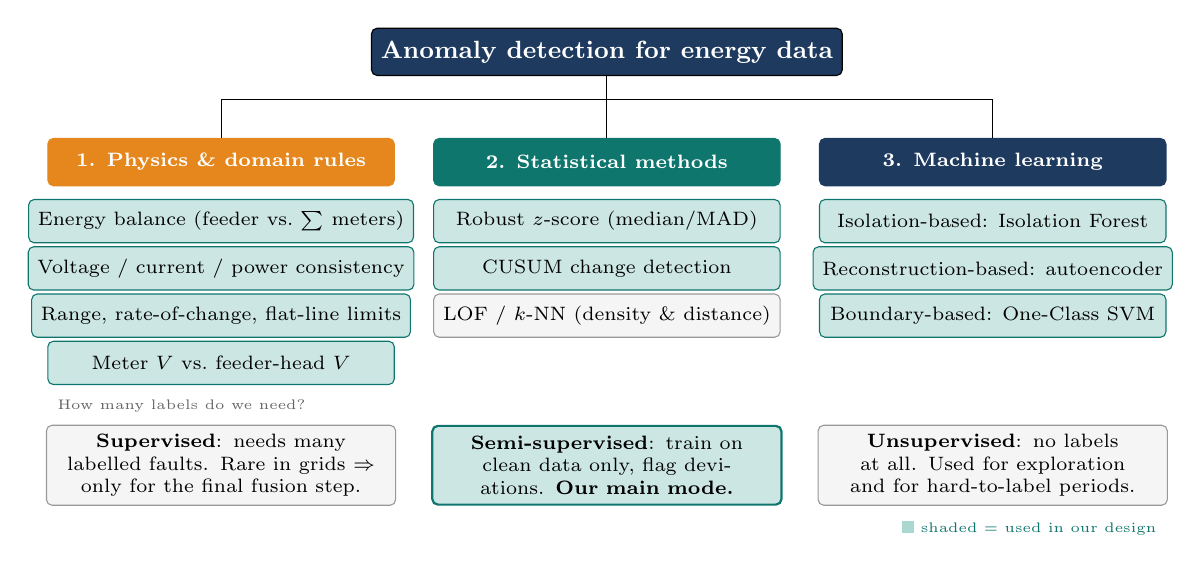
\begin{tikzpicture}[
  fam/.style={draw,rounded corners=2pt,text=white,font=\scriptsize\bfseries,minimum width=44mm,minimum height=6mm},
  used/.style={draw=mzteal,fill=good!60,rounded corners=2pt,font=\scriptsize,minimum width=44mm,minimum height=5.5mm},
  unused/.style={draw=black!40,fill=black!4,rounded corners=2pt,font=\scriptsize,minimum width=44mm,minimum height=5.5mm},
  lab/.style={draw,rounded corners=2pt,font=\scriptsize,align=center,text width=42mm,minimum height=10mm}]
\node[fam,fill=mznavy,minimum width=44mm,font=\small\bfseries] (root) at (4.9,1.4) {Anomaly detection for energy data};
\node[fam,fill=mzorange,draw=mzorange] (f1) at (0,0) {1. Physics \& domain rules};
\node[fam,fill=mzteal,draw=mzteal] (f2) at (4.9,0) {2. Statistical methods};
\node[fam,fill=mznavy,draw=mznavy] (f3) at (9.8,0) {3. Machine learning};
\draw (root.south)--(4.9,0.8); \draw (0,0.8)--(9.8,0.8);
\foreach \f in {f1,f2,f3}{\draw (\f.north|-0,0.8)--(\f.north);}
\node[used] at (0,-0.75) {Energy balance (feeder vs.\ $\sum$ meters)};
\node[used] at (0,-1.35) {Voltage / current / power consistency};
\node[used] at (0,-1.95) {Range, rate-of-change, flat-line limits};
\node[used] at (0,-2.55) {Meter $V$ vs.\ feeder-head $V$};
\node[used] at (4.9,-0.75) {Robust $z$-score (median/MAD)};
\node[used] at (4.9,-1.35) {CUSUM change detection};
\node[unused] at (4.9,-1.95) {LOF / $k$-NN (density \& distance)};
\node[used] at (9.8,-0.75) {Isolation-based: Isolation Forest};
\node[used] at (9.8,-1.35) {Reconstruction-based: autoencoder};
\node[used] at (9.8,-1.95) {Boundary-based: One-Class SVM};
\node[font=\tiny,anchor=west,text=black!60] at (-2.2,-3.1) {How many labels do we need?};
\node[lab,draw=black!40,fill=black!4] at (0,-3.85) {\textbf{Supervised}: needs many labelled faults. Rare in grids $\Rightarrow$ only for the final fusion step.};
\node[lab,draw=mzteal,fill=good!60,thick] at (4.9,-3.85) {\textbf{Semi-supervised}: train on clean data only, flag deviations. \textbf{Our main mode.}};
\node[lab,draw=black!40,fill=black!4] at (9.8,-3.85) {\textbf{Unsupervised}: no labels at all. Used for exploration and for hard-to-label periods.};
\node[font=\tiny,text=mzteal,anchor=east] at (12,-4.65) {\textcolor{good}{\rule{1.5mm}{1.5mm}} shaded = used in our design};
\end{tikzpicture}
\caption{Taxonomy of detectors. Teal boxes are the methods we use (detailed in Section~\ref{sec:methods}).
Hybrid physics\,+\,learning follows the argument that high-stakes decisions should rest on inspectable models
where possible~\cite{rudin}.}
\label{fig:taxonomy}
\end{figure}

% =====================================================================
\section{The Methods, One by One}
\label{sec:methods}

\subsection{Statistical Outlier Methods}
\paragraph{Robust $z$-score.} The classic $z=(x-\bar x)/s$ is distorted by the very outliers it seeks,
because mean and standard deviation have a 0\% breakdown point. Replacing them by the median and the scaled
median absolute deviation gives
\begin{equation}
  z_i^{\mathrm{rob}}=\frac{x_i-\operatorname{med}(x)}{1.4826\cdot\mathrm{MAD}(x)},\qquad
  \mathrm{MAD}=\operatorname{med}_i\lvert x_i-\operatorname{med}(x)\rvert,
\end{equation}
which tolerates up to 50\% contamination~\cite{rousseeuw,leys}. \textbf{CUSUM}~\cite{page} accumulates small
deviations, $S_t=\max\bigl(0,\,S_{t-1}+(x_t-\mu_0)/\sigma-k\bigr)$, and alarms when $S_t>h$; it is the
natural tool for slow drift. \textbf{LOF}~\cite{lof} compares a point's local density with that of its
neighbours, so it handles clusters of different density.

\begin{figure}[H]
\centering
\begin{tikzpicture}
\begin{groupplot}[group style={group size=2 by 1,horizontal sep=14mm},
  width=7.4cm,height=4.6cm,tick label style={font=\tiny},label style={font=\scriptsize},
  title style={font=\scriptsize\bfseries},grid=major,grid style={black!10},
  legend style={font=\tiny,draw=none,fill=white,fill opacity=0.8,text opacity=1},xlabel={sample index}]
\nextgroupplot[title={Masking: ordinary vs.\ robust $z$},ylabel={$\lvert z\rvert$},
  xmin=-2,xmax=66,ymin=0,ymax=14,legend pos=north west]
  \addplot[only marks,mark=o,mark size=1.1pt,black!45,forget plot] table[x=i,y=z]{data/mask_normal.dat};
  \addplot[only marks,mark=diamond*,mark size=1.8pt,mzorange] table[x=i,y=zord]{data/mask_out.dat};
  \addlegendentry{ordinary $z$}
  \addplot[only marks,mark=triangle*,mark size=2pt,mzteal] table[x=i,y=zrob]{data/mask_out.dat};
  \addlegendentry{robust $z$}
  \addplot[mzred,dashed,thick,domain=-2:66] {3};
  \addlegendentry{threshold 3}
\nextgroupplot[title={CUSUM catches a $1\sigma$ mean shift},xmin=0,xmax=160,ymin=-3,ymax=12,
  legend pos=north west]
  \addplot[black!35,thin] table[x=i,y=x]{data/cusum.dat}; \addlegendentry{signal}
  \addplot[mzteal,thick] table[x=i,y=S]{data/cusum.dat}; \addlegendentry{$S_t$}
  \addplot[mzred,dashed,thick,domain=0:160] {4}; \addlegendentry{$h=4$}
  \addplot[only marks,mark=*,mark size=1.6pt,mzred,forget plot] table[x=i,y=S]{data/cusum_alarm.dat};
  \draw[mznavy,densely dotted,thick] (axis cs:80,-3)--(axis cs:80,12);
  \node[font=\tiny,text=mznavy,anchor=south west] at (axis cs:81,-2.8) {shift at 80};
\end{groupplot}
\end{tikzpicture}
\caption{Left: four injected outliers among 60 normal samples. Ordinary $z$ gives \zOrd, so
\zOrdHidden{} of them hides below the threshold (masking); robust $z$ gives \zRob, so all four are flagged.
Right: CUSUM ($k=0.5$, $h=4$) alarms at sample \cusumAlarm, \cusumDelay{} samples after the shift, although the
raw signal stays mostly within $\pm3\sigma$. Both from our \texttt{gen.py}, synthetic data, fixed seed.}
\label{fig:stat}
\end{figure}

\paragraph{Role in our design.} Cheap, transparent first line and the baseline every ML component must beat.
Robust $z$ is applied to residuals from each meter's own 28-day half-hourly profile, so the evening peak,
weekends, Ramadan and heat-wave days are not mistaken for anomalies. CUSUM runs on two slow signals: the
meter's voltage relative to its feeder head (a sensor offset) and the feeder's daily energy-balance gap
(a bias or bypass somewhere on the feeder).

\paragraph{The physics rules and what they cannot see.} The rule $E\approx V I\cos\varphi\,\Delta t$ exposes
\emph{data-only} injection, which edits the energy field and leaves $V$ and $I$ untouched. It is skipped while
a meter exports PV energy (import is then 0 while current flows; without the gate it fires on 39\% of the clean
readings of N1's PV homes). It is \emph{blind} to sensor bias, gain drift and physical bypass, which scale
energy and current together, so those cases rest on the feeder balance and on the meter's own history.
A meter cannot read a higher voltage than the head of its feeder, because voltage only drops along the line;
a persistent excess (24-h median above $+1.5$~V, export readings excluded) is a voltage-sensor offset.

\subsection{Isolation Forest}
Liu, Ting and Zhou~\cite{iforest} observed that anomalies are few and different, so random axis-parallel
cuts isolate them in fewer splits. A tree is grown by repeatedly picking a random feature and a random split
value; the path length $h(x)$ to isolate $x$ is short for anomalies. With subsample size $\psi$ the score is
\begin{equation}
  s(x,\psi)=2^{-E[h(x)]/c(\psi)},\qquad c(\psi)=2H(\psi-1)-\frac{2(\psi-1)}{\psi},\qquad H(i)\approx\ln i+0.5772,
\end{equation}
so $s\to1$ for anomalies and $s<0.5$ for normal points. It is linear in time, needs no labels and no distance
computations. The Extended Isolation Forest uses randomly oriented cuts and removes the axis-parallel
artefacts visible in score maps~\cite{eif}, which matters for correlated quantities such as $V$ and $I$.

\begin{figure}[H]
\centering
\begin{minipage}{0.6\textwidth}
\centering
\begin{tikzpicture}
\begin{axis}[width=\linewidth,height=5cm,ybar,bar width=4pt,
  title={Why it works: path length to isolate a point},title style={font=\scriptsize\bfseries},
  tick label style={font=\tiny},label style={font=\scriptsize},
  xlabel={mean path length over 200 trees},ylabel={density},xmin=2,xmax=14.5,ymin=0,
  grid=major,grid style={black!10},legend style={font=\tiny,draw=none,at={(0.03,0.97)},anchor=north west}]
  \addplot[draw=mznavy,fill=mznavy!35] table[x=mid,y=normal]{data/pathlen.dat}; \addlegendentry{normal points}
  \addplot[draw=mzred,fill=mzred!45] table[x=mid,y=anom]{data/pathlen.dat}; \addlegendentry{anomalies}
\end{axis}
\end{tikzpicture}
\end{minipage}\hfill
\begin{minipage}{0.36\textwidth}
\small\textbf{Reading the plot.} Normal points sit deep inside dense regions, so many random cuts are
needed to separate them (mean $\approx$ \pathNormal). Anomalies are isolated after only \pathAnom{} cuts on
average. A short average path means a high score $s$. Same kind of 2-D cloud as Figure~\ref{fig:maps}.
\end{minipage}
\caption{Average isolation path length from the fitted Isolation Forest (200 trees; 250 normal points and
250 anomalies drawn outside the dense core).}
\label{fig:pathlen}
\end{figure}

\subsection{One-Class SVM}
Schölkopf et al.~\cite{ocsvm} separate the data from the origin in a kernel feature space with maximum margin:
\begin{equation}
  \min_{w,\xi,\rho}\ \tfrac12\lVert w\rVert^2+\frac{1}{\nu n}\sum_i\xi_i-\rho
  \quad\text{s.t.}\quad \langle w,\phi(x_i)\rangle\ge\rho-\xi_i,\ \ \xi_i\ge0,
\end{equation}
and $f(x)=\operatorname{sgn}\bigl(\langle w,\phi(x)\rangle-\rho\bigr)$ with an RBF kernel. The parameter $\nu$
upper-bounds the fraction of training points treated as outliers. The closely related SVDD~\cite{svdd}
encloses the data in a minimal hypersphere.

\begin{figure}[H]
\centering
\begin{tikzpicture}
\begin{groupplot}[group style={group size=2 by 1,horizontal sep=22mm},
  width=6.6cm,height=5.4cm,tick label style={font=\tiny},label style={font=\scriptsize},
  title style={font=\scriptsize\bfseries},xmin=-6,xmax=6,ymin=-5.5,ymax=5.5,
  xlabel={feature 1},enlargelimits=false,axis on top,
  colorbar style={width=2.5mm,tick label style={font=\tiny}}]
\nextgroupplot[title={Isolation Forest: anomaly score $s$},ylabel={feature 2},
  colormap/ifmap,colorbar,point meta min=\ifSMin,point meta max=\ifSMax]
  \addplot graphics[xmin=-6,xmax=6,ymin=-5.5,ymax=5.5] {data/if_map.png};
  \addplot[only marks,mark=*,mark size=0.6pt,mznavy!80] table{data/cloud.dat};
  \addplot[only marks,mark=x,mark size=2.5pt,very thick,black] table{data/outliers.dat};
\nextgroupplot[title={One-Class SVM: decision value $f$},colormap/svmmap,colorbar,
  point meta min=-1,point meta max=1]
  \addplot graphics[xmin=-6,xmax=6,ymin=-5.5,ymax=5.5] {data/svm_map.png};
  \addplot[only marks,mark=*,mark size=0.6pt,mznavy!80] table{data/cloud.dat};
  \addplot[only marks,mark=x,mark size=2.5pt,very thick,black] table{data/outliers.dat};
\end{groupplot}
\end{tikzpicture}
\caption{Two detectors fitted by \texttt{scikit-learn}~\cite{sklearn} on the same correlated 2-D ``normal''
cloud (blue dots); crosses are injected outliers. Isolation Forest (200 trees, $\psi=256$) scores the outliers
\ifOutMin--\ifOutMax{} against a mean of \ifNormMean{} for normal points. The One-Class SVM ($\nu=0.05$, RBF;
decision value scaled to $[-1,1]$) draws a smooth boundary (white) around the data. Their different inductive
biases are why disagreement carries information.}
\label{fig:maps}
\end{figure}

\paragraph{Role in our design.} Both run on daily window features of each meter (48 readings): profile residual
(mean, maximum, spread), change of the meter's share against its feeder neighbours, physics ratio, $V$ minus
feeder-head $V$, share of zero readings, longest frozen run, lag gain against the profile (clock shift),
similarity to the same day a week earlier (replay), distortion and minimum/maximum voltage. Isolation Forest is our fast first ML pass. OCSVM is trained on a
subsample (it scales poorly) as a second, differently-biased opinion. When they disagree, confidence drops
and the case is routed to a human.

\subsection{Autoencoders}
An autoencoder learns to compress and reconstruct normal data through a narrow code. Trained on clean data
only, it reconstructs anomalies badly, so the reconstruction error is the anomaly score~\cite{sakurada}:
\begin{equation}
  e(x)=\lVert x-g(f(x))\rVert^2=\textstyle\sum_j e_j,\qquad e_j=(x_j-\hat x_j)^2.
\end{equation}
LSTM encoder--decoders extend this to multi-sensor time series~\cite{malhotra}; surveys of deep detectors
discuss when they help and where they over-generalise and reconstruct anomalies too well~\cite{pang}.
Crucially for us, the \emph{per-channel} error $e_j$ points at \emph{which sensor} looks wrong, and it can be
fed to Shapley-value explanations~\cite{shap}.

\begin{figure}[H]
\centering
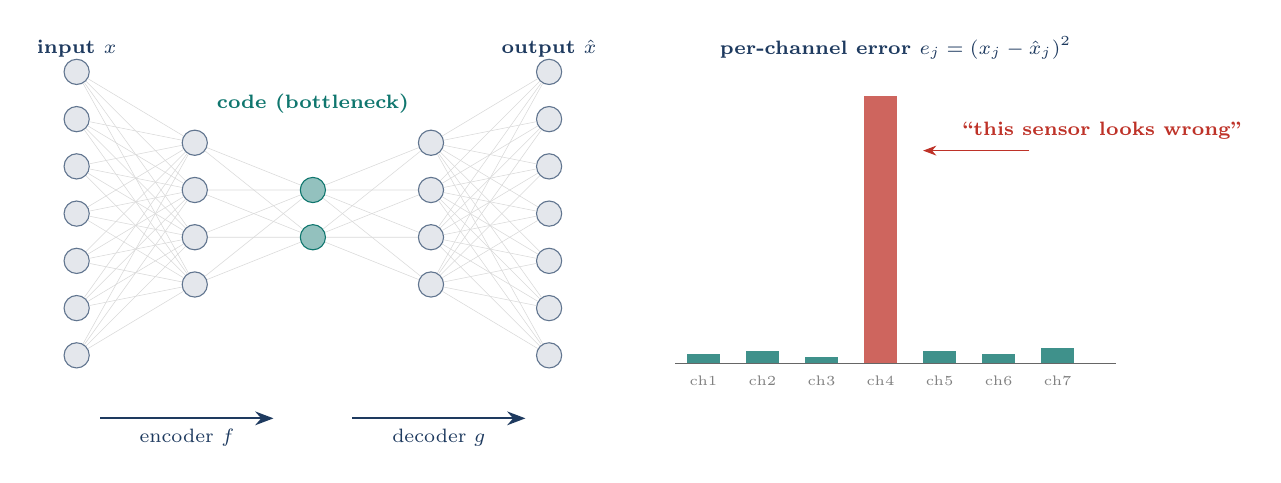
\begin{tikzpicture}[n/.style={circle,draw=mznavy!70,fill=mznavy!12,minimum size=3.2mm,inner sep=0pt},
  c/.style={circle,draw=mzteal,fill=mzteal!45,minimum size=3.2mm,inner sep=0pt}]
\foreach \i in {1,...,7}{\node[n] (a\i) at (0,1.8-0.6*\i+0.6) {}; \node[n] (e\i) at (6,1.8-0.6*\i+0.6) {};}
\foreach \i in {1,...,4}{\node[n] (b\i) at (1.5,1.2-0.6*\i+0.3) {}; \node[n] (d\i) at (4.5,1.2-0.6*\i+0.3) {};}
\foreach \i in {1,2}{\node[c] (c\i) at (3,0.6-0.6*\i+0.3) {};}
\begin{scope}[on background layer/.style={},black!15,very thin]
\foreach \i in {1,...,7}{\foreach \j in {1,...,4}{\draw (a\i)--(b\j); \draw (d\j)--(e\i);}}
\foreach \i in {1,...,4}{\foreach \j in {1,2}{\draw (b\i)--(c\j); \draw (c\j)--(d\i);}}
\end{scope}
\node[font=\scriptsize\bfseries,text=mznavy] at (0,2.1) {input $x$};
\node[font=\scriptsize\bfseries,text=mznavy] at (6,2.1) {output $\hat x$};
\node[font=\scriptsize\bfseries,text=mzteal] at (3,1.4) {code (bottleneck)};
\draw[mznavy,thick,-{Stealth}] (0.3,-2.6)--(2.5,-2.6) node[midway,below,font=\scriptsize] {encoder $f$};
\draw[mznavy,thick,-{Stealth}] (3.5,-2.6)--(5.7,-2.6) node[midway,below,font=\scriptsize] {decoder $g$};
% per-channel error bars (illustrative values)
\begin{scope}[xshift=7.6cm,yshift=-1.9cm]
\node[font=\scriptsize\bfseries,text=mznavy] at (2.8,4.0) {per-channel error $e_j=(x_j-\hat x_j)^2$};
\draw[black!60] (0,0)--(5.6,0);
\foreach \k/\h in {1/0.12,2/0.15,3/0.08,4/3.4,5/0.15,6/0.12,7/0.19}{
  \ifnum\k=4 \fill[mzred!75] (\k*0.75-0.6,0) rectangle ++(0.42,\h);
  \else \fill[mzteal!80] (\k*0.75-0.6,0) rectangle ++(0.42,\h); \fi
  \node[font=\tiny,text=black!50] at (\k*0.75-0.39,-0.22) {ch\k};}
\draw[mzred,-{Stealth}] (4.5,2.7)--(3.15,2.7);
\node[font=\scriptsize\bfseries,text=mzred,anchor=west] at (3.5,2.95) {``this sensor looks wrong''};
\end{scope}
\end{tikzpicture}
\caption{Autoencoder principle (left) and the per-channel reconstruction error that localises the faulty
sensor (right; illustrative values).}
\label{fig:ae}
\end{figure}

\paragraph{Role in our design.} Trained on clean windows only; captures correlated-sensor inconsistencies and
subtle waveform changes that thresholds miss, and gives channel-level evidence for the explanation sentence
(``channel 4 deviates most'').

\subsection{The Methods at a Glance}
\begin{table}[H]
\centering
\small
\renewcommand{\arraystretch}{1.15}
\begin{tabularx}{\textwidth}{@{}>{\raggedright\arraybackslash}p{2.3cm}>{\raggedright\arraybackslash}p{1.2cm}>{\raggedright\arraybackslash}p{1.8cm}>{\raggedright\arraybackslash}p{2.2cm}LL@{}}
\toprule
\textbf{Method} & \textbf{Labels} & \textbf{Run cost} & \textbf{Explainable} & \textbf{Strong on} & \textbf{Weak on} \\
\midrule
Rules / physics & \cellcolor{good}none & \cellcolor{good}very low & \cellcolor{good}by design & Impossible values, data-only injection, voltage offset & Bias and bypass (physics still holds) \\
Robust $z$ / CUSUM & \cellcolor{good}none & \cellcolor{good}very low & \cellcolor{good}high & Spikes; persistent offsets & Seasonal baselines (feeder balance) \\
Isolation Forest & \cellcolor{good}none & \cellcolor{good}low & \cellcolor{fair}medium (TreeSHAP) & Global outliers, many features & Shifts inside the normal range \\
One-Class SVM & \cellcolor{good}none & \cellcolor{poor}high on big data & \cellcolor{poor}low (post-hoc) & Smooth boundary on compact data & Scale; kernel tuning \\
Autoencoder & \cellcolor{good}none & \cellcolor{fair}medium (training) & \cellcolor{fair}medium (per channel) & Correlated-sensor, waveform change & Can reconstruct anomalies too well \\
\bottomrule
\end{tabularx}
\caption{Qualitative comparison, our assessment from the cited literature~\cite{chandola,pang} and the
experiment in Section~\ref{sec:experiment}. Green = favourable, amber = acceptable, red = costly.}
\label{tab:glance}
\end{table}

% =====================================================================
\section{Putting It Together: Our Hybrid Detection Stack}
\label{sec:stack}

\begin{figure}[H]
\centering
\resizebox{\textwidth}{!}{%
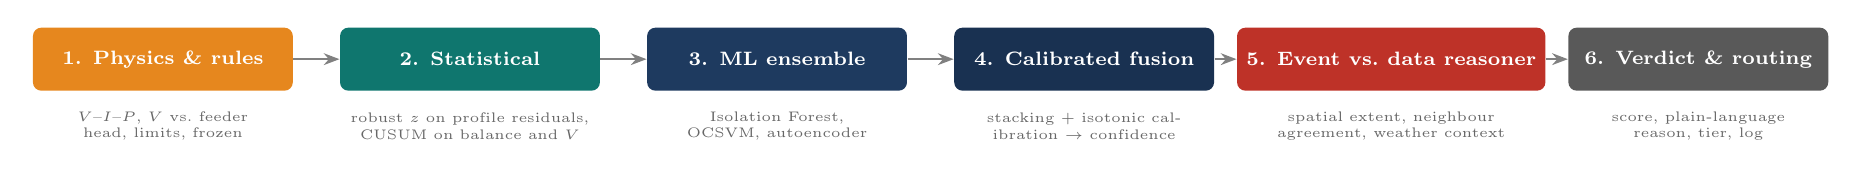
\begin{tikzpicture}[
  st/.style={rounded corners=3pt,text=white,font=\scriptsize\bfseries,minimum width=33mm,minimum height=8mm,align=center},
  sub/.style={font=\tiny,text=black!60,align=center,text width=32mm},
  >={Stealth[length=2mm]}]
\foreach \i/\name/\col/\txt in {
  1/1. Physics \& rules/mzorange/{$V$--$I$--$P$, $V$ vs.\ feeder head, limits, frozen},
  2/2. Statistical/mzteal/{robust $z$ on profile residuals, CUSUM on balance and $V$},
  3/3. ML ensemble/mznavy/{Isolation Forest,\\ OCSVM, autoencoder},
  4/4. Calibrated fusion/mznavy!85!black/{stacking + isotonic calibration $\rightarrow$ confidence},
  5/5. Event vs.\ data reasoner/mzred/{spatial extent, neighbour agreement, weather context},
  6/6. Verdict \& routing/black!65/{score, plain-language reason, tier, log}}{
  \node[st,fill=\col] (s\i) at (\i*3.9,0) {\name};
  \node[sub] at (\i*3.9,-0.85) {\txt};}
\foreach \a/\b in {1/2,2/3,3/4,4/5,5/6}{\draw[->,black!50,thick] (s\a)--(s\b);}
\end{tikzpicture}}
\caption{The detection pipeline. Rules can veto or force escalation; ML scores add sensitivity; the
reasoner decides \emph{what kind} of unusual it is.}
\label{fig:stack}
\end{figure}

\paragraph{How the verdict is reached.} Layers 1--3 answer ``is something unusual?'' and are \emph{meant} to
fire on genuine events too; layer 5 answers ``what kind?'' from consistency features
(Table~\ref{tab:reasoner}). Layers 5--6 are specified in the Goal~2 and Goal~3 notes; this note covers
layers 1--4.

\begin{table}[H]
\centering
\small
\begin{tabularx}{0.85\textwidth}{@{}>{\raggedright\arraybackslash}p{5cm}LL@{}}
\toprule
\textbf{Evidence} & \textbf{Genuine event} & \textbf{Data-quality problem} \\
\midrule
Spatial extent (meters affected) & Many & One or a few \\
Physical consistency ($V$, $I$, $P$) & Holds & Violated (data-only injection) or holds (bias, bypass) \\
Feeder energy balance & Unchanged & Opens (under-reporting) or goes negative (inflation) \\
Supply & $V=0$ on many meters (outage) & $V>0$ \\
Agreement with correlated neighbours & Yes & Contradicts them \\
Temporal shape & Physical dynamics & Step, frozen, replayed \\
Weather / time-of-day context & Explains it & Does not explain it \\
\bottomrule
\end{tabularx}
\caption{Consistency features used by the event-versus-data reasoner.}
\label{tab:reasoner}
\end{table}

\subsection{Results on Node N1 of the Challenge Dataset}
\label{sec:experiment}
\paragraph{Set-up.} Unit of analysis: one meter-day (48 readings) of node N1, from 8~January (the profiles need
one week of history) to 31~December, excluding days that are mostly missing: \nOneDays{} meter-days, of which
\nOneClean{} are clean and the rest belong to \nOneEvents{} labelled events. Every detector is trained on clean
meter-days only; labels are used only to score. Thresholds give a 1\% false-positive rate on held-out clean
days (the stack: rules, or any learned detector at 0.25\%). Everything is out-of-fold over 5~folds, with clean
days grouped by meter-week and anomalous days grouped by event, so no event is split. A time split is not
possible: in N1, November--December contain no falsification and no sensor-bias event. An event counts as
\emph{detected} when at least 20\% of its meter-days are flagged (any flag for events of five days or less),
so a long event is not ``caught'' by a chance alarm. Code: \texttt{n1\_experiment.py}.

\begin{table}[H]
\centering
\small
\setlength{\tabcolsep}{4pt}
\begin{tabular}{@{}l cc cc cc |c@{}}
\toprule
 & \multicolumn{2}{c}{\textbf{Genuine event}} & \multicolumn{2}{c}{\textbf{Meter fault}} & \multicolumn{2}{c|}{\textbf{Falsification}} & \textbf{False} \\
\textbf{Detector} & days & events & days & events & days & events & \textbf{positives} \\
\midrule
% generated by n1_experiment.py
Rules (layer 1) & \hc{42} & 17/36 & \hc{29} & 18/30 & \hc{66} & 5/8 & 0.0\% \\
Robust z & \hc{1} & 3/36 & \hc{26} & 12/30 & \hc{61} & 5/8 & 1.1\% \\
CUSUM & \hc{1} & 4/36 & \hc{12} & 2/30 & \hc{6} & 0/8 & 2.1\% \\
Isolation Forest & \hc{3} & 11/36 & \hc{7} & 15/30 & \hc{9} & 2/8 & 0.9\% \\
One-Class SVM & \hc{74} & 30/36 & \hc{31} & 25/30 & \hc{67} & 6/8 & 1.3\% \\
Autoencoder & \hc{74} & 30/36 & \hc{28} & 22/30 & \hc{64} & 5/8 & 1.1\% \\
Detection stack & \hc{74} & 30/36 & \hc{31} & 23/30 & \hc{69} & 6/8 & 2.3\% \\
\bottomrule
% ends with \bottomrule
\end{tabular}
\caption{Node N1, out-of-fold. ``days'': share (\%) of the class's meter-days flagged (darker = higher).
``events'': events detected / events. False positives: share of clean meter-days flagged. Genuine events:
outage, load shedding, sag, swell, surge, cable fault, transformer; meter faults: corruption and sensor faults;
falsification: the 8 manipulation types. Simulated data.}
\label{tab:experiment}
\end{table}

\begin{table}[H]
\centering
\small
\setlength{\tabcolsep}{4pt}
\resizebox{\textwidth}{!}{%
\begin{tabular}{@{}l c c r l l r l@{}}
\toprule
\textbf{Event (N1)} & \textbf{Feeder} & \textbf{Start} & \textbf{Days} & \textbf{Detected by} & \textbf{First flag} & \textbf{Days flagged} & \textbf{Balance alarm} \\
\midrule
% generated by n1_experiment.py
\texttt{partial\_reduction\_bypass} & F2 & 04 Feb & 60 & -- & day 8 & 18\% & day 13 \\
\texttt{selective\_bypass} & F2 & 09 Feb & 65 & -- & day 3 & 5\% & day 8 \\
\texttt{meter\_zeroing} & F1 & 11 May & 20 & IF, SVM & day 0 & 22\% & -- \\
\texttt{fdi\_scale} & F3 & 02 May & 63 & R, z, SVM, AE & day 1 & 98\% & day 14 \\
\texttt{fdi\_evasion} & F2 & 25 Apr & 35 & R, z, IF, SVM, AE & day 0 & 100\% & day 9 \\
\texttt{fdi\_inflate} & F3 & 12 Sep & 33 & R, z, SVM, AE & day 1 & 97\% & day 13 \\
\texttt{fdi\_replay} & F2 & 09 Aug & 29 & R, z, SVM, AE & day 0 & 100\% & -- \\
\texttt{coordinated\_fdi} & F1 & 14 Oct & 26 & R, z, SVM, AE & day 0 & 100\% & day 6 \\
\texttt{bias\_step} & F1 & 05 Jun & 58 & -- & day 2 & 5\% & day 14 \\
\texttt{gain\_drift} & F2 & 19 Apr & 66 & -- & -- & 0\% & day 15 \\
\texttt{gain\_drift} & F2 & 18 May & 65 & -- & day 42 & 2\% & day 16 \\
\texttt{clock\_shift} & F1 & 23 Feb & 15 & -- & -- & 0\% & -- \\
\texttt{voltage\_offset\_drift} & F1 & 10 Apr & 64 & R, z, C, SVM, AE & day 0 & 100\% & day 3 \\
\texttt{stuck\_value} & F1 & 12 Feb & 3 & R, z, IF, SVM, AE & day 0 & 100\% & -- \\
\texttt{stuck\_value} & F2 & 28 Jun & 1 & R, z, IF, SVM, AE & day 0 & 100\% & -- \\
\texttt{stuck\_value} & F3 & 10 Nov & 2 & -- & -- & 0\% & -- \\
\bottomrule
% ends with \bottomrule
\end{tabular}}
\caption{The \nRare{} falsification and sensor-fault events of N1, one by one (most types occur once, so
percentages per type would be meaningless). R = rules, z = robust $z$, C = CUSUM, IF, SVM, AE = autoencoder.
First flag and days flagged refer to the whole stack. Balance alarm: first day the CUSUM on the feeder's daily
energy-balance gap fires (it is in alarm on \balFPR\% of clean feeder-days); it names a feeder, not a meter.}
\label{tab:events}
\end{table}

\needspace{8\baselineskip}
\paragraph{What the results show.}
\begin{itemize}[leftmargin=*,itemsep=2pt]
  \item \textbf{The stack is usable as a first filter.} It flags \stackFPR\% of clean meter-days. The physics
        and domain rules alone flag none, yet they catch every data-only injection, the voltage offset and two of
        the three stuck meters from the first or second day (the third froze for 4~hours across midnight,
        below the 3-hour-per-day limit on either side).
  \item \textbf{No detector wins everywhere.} The One-Class SVM and the autoencoder carry the learned part
        (about three quarters of genuine-event days, most meter-fault events). Robust $z$ is strong on
        falsification days but blind to genuine events. Isolation Forest is weak at this false-positive rate:
        most anomalies here shift values \emph{inside} the normal range rather than isolate them.
  \item \textbf{The hard cases are the physically consistent ones.} Partial and selective bypass, the
        constant bias and both gain drifts keep $V$, $I$ and $E$ consistent and are flagged on at most 18\% of
        their days, as is a clock shift. This matches the difficulty ranking published with the dataset.
  \item \textbf{The feeder balance sees them, but only as a feeder.} Its CUSUM fires 8--16 days after the start
        of both bypasses, the bias and both drifts. Pointing to the right meter fails: a household's daily
        share of its feeder varies far more than a 7--14\% bias, and the gap itself moves: about \gapSd{}~points of
        day-to-day noise on clean days, plus a spring--summer drop when PV homes export. Phase~2 will model
        the expected gap from feeder load, PV export and temperature, run CUSUM on the residual, and attribute
        alarms with longer windows.
  \item \textbf{Limits.} Simulated data from one generator; most falsification and sensor types occur once in
        N1, so these are case results, not rates. Feeder-level references use clean feeder-days.
\end{itemize}

\subsection{Output to the Explanation Layer (Goal 2)}
For every flagged meter-day, the detection layer passes on: the stack decision and each detector's score; which rules
fired, with the measured value and threshold; the neighbourhood support (share of the feeder's 10 meters flagged
the same day); the feeder-balance alarm state; and the autoencoder's per-feature reconstruction error, which
tells Goal~2 which channel looks wrong.

% =====================================================================
\begin{thebibliography}{99}
\bibitem{chandola} V.~Chandola, A.~Banerjee and V.~Kumar, ``Anomaly detection: A survey,'' \emph{ACM Computing Surveys}, vol.~41, no.~3, 2009.
\bibitem{pang} G.~Pang, C.~Shen, L.~Cao and A.~van den Hengel, ``Deep learning for anomaly detection: A review,'' \emph{ACM Computing Surveys}, vol.~54, no.~2, 2021.
\bibitem{fdi} Y.~Liu, P.~Ning and M.~K.~Reiter, ``False data injection attacks against state estimation in electric power grids,'' \emph{ACM Trans.\ Information and System Security}, vol.~14, no.~1, 2011.
\bibitem{rudin} C.~Rudin, ``Stop explaining black box machine learning models for high stakes decisions and use interpretable models instead,'' \emph{Nature Machine Intelligence}, vol.~1, pp.~206--215, 2019.
\bibitem{rousseeuw} P.~J.~Rousseeuw and C.~Croux, ``Alternatives to the median absolute deviation,'' \emph{J.\ American Statistical Association}, vol.~88, no.~424, 1993.
\bibitem{leys} C.~Leys, C.~Ley, O.~Klein, P.~Bernard and L.~Licata, ``Detecting outliers: Do not use standard deviation around the mean, use absolute deviation around the median,'' \emph{J.\ Experimental Social Psychology}, vol.~49, no.~4, 2013.
\bibitem{page} E.~S.~Page, ``Continuous inspection schemes,'' \emph{Biometrika}, vol.~41, no.~1/2, 1954.
\bibitem{lof} M.~M.~Breunig, H.-P.~Kriegel, R.~T.~Ng and J.~Sander, ``LOF: Identifying density-based local outliers,'' in \emph{Proc.\ ACM SIGMOD}, 2000.
\bibitem{iforest} F.~T.~Liu, K.~M.~Ting and Z.-H.~Zhou, ``Isolation Forest,'' in \emph{Proc.\ IEEE ICDM}, 2008.
\bibitem{eif} S.~Hariri, M.~Carrasco Kind and R.~J.~Brunner, ``Extended Isolation Forest,'' \emph{IEEE Trans.\ Knowledge and Data Engineering}, vol.~33, no.~4, 2021.
\bibitem{ocsvm} B.~Schölkopf, J.~C.~Platt, J.~Shawe-Taylor, A.~J.~Smola and R.~C.~Williamson, ``Estimating the support of a high-dimensional distribution,'' \emph{Neural Computation}, vol.~13, no.~7, 2001.
\bibitem{svdd} D.~M.~J.~Tax and R.~P.~W.~Duin, ``Support vector data description,'' \emph{Machine Learning}, vol.~54, 2004.
\bibitem{sakurada} M.~Sakurada and T.~Yairi, ``Anomaly detection using autoencoders with nonlinear dimensionality reduction,'' in \emph{Proc.\ MLSDA Workshop}, 2014.
\bibitem{malhotra} P.~Malhotra, A.~Ramakrishnan, G.~Anand, L.~Vig, P.~Agarwal and G.~Shroff, ``LSTM-based encoder-decoder for multi-sensor anomaly detection,'' ICML Anomaly Detection Workshop, arXiv:1607.00148, 2016.
\bibitem{shap} S.~M.~Lundberg and S.-I.~Lee, ``A unified approach to interpreting model predictions,'' in \emph{Advances in Neural Information Processing Systems}, 2017.
\bibitem{sklearn} F.~Pedregosa et al., ``Scikit-learn: Machine learning in Python,'' \emph{J.\ Machine Learning Research}, vol.~12, 2011.
\end{thebibliography}
\end{document}
